% !TeX TS-program = xelatex

\documentclass{resume}
\ResumeName{张硕}

% 如果想插入照片，请使用以下两个库。
\usepackage{graphicx}
\usepackage{tikz}

\begin{document}

\ResumeContacts{
  % \ResumeUrl{mailto:zhang.shuo@bupt.edu.cn}{zhang.shuo@bupt.edu.cn},%
  出生日期: 2002.04.28,
  性别: 男,
  民族: 汉族,
  籍贯: 山东济宁,%
  电话: 153-3547-0446%
}

% 如果想插入照片，请取消此代码的注释。
% 但是默认不推荐插入照片，因为这不是简历的重点。
% 如果默认的照片插入格式不能满足你的需求，你可以尝试调整照片的大小，或者使用其他的插入照片的方法。
% 不然，也可以先渲染 PDF 简历，然后用其他工具在 PDF 上叠加照片。
%begin{tikzpicture}[remember picture, overlay]
%  \node [anchor=north east, inner sep=1cm] at (current page.north east)  
%     {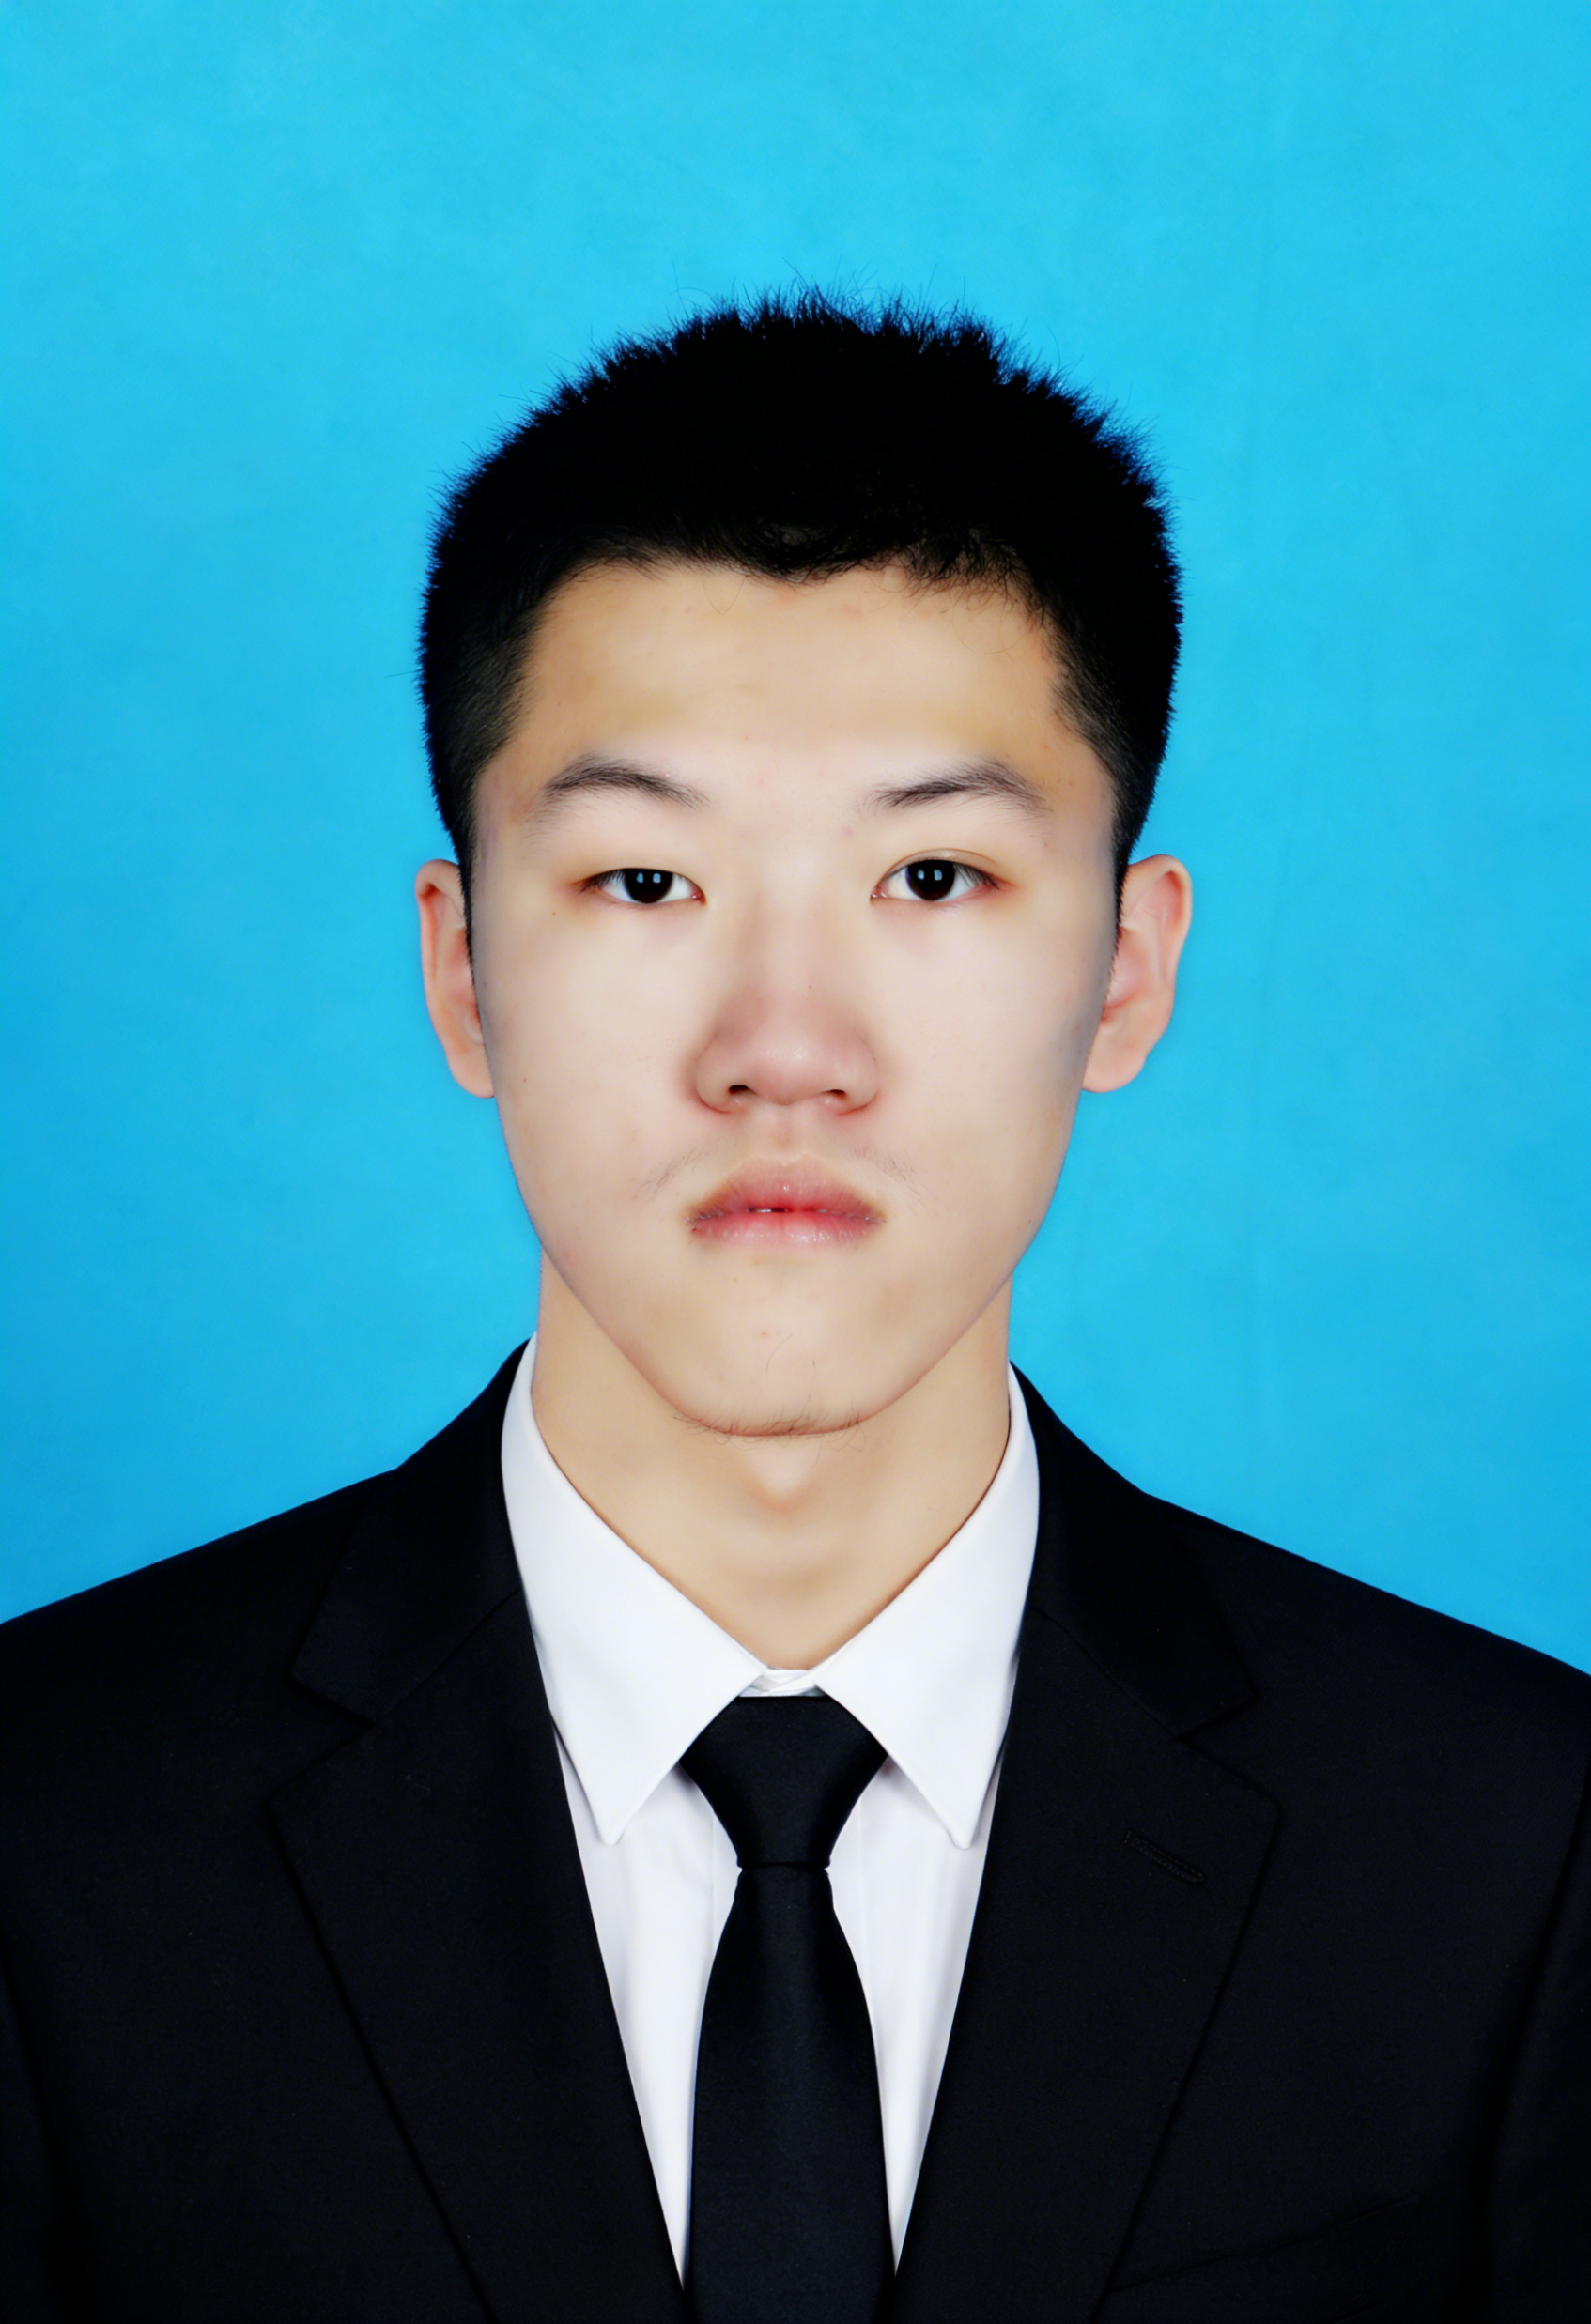
\includegraphics[width=2cm]{image.png}};
%\end{tikzpicture}

\ResumeTitle

\section{政治表现}
\begin{itemize}
	\item \textbf{政治面貌:} 2017 年 6 月成为\textbf{共青团员}，团龄 9 年；2023 年 5 月成为\textbf{中共党员}，党龄3年。
	\item \textbf{政治立场:} 在校期间长期参与党内理论学习，带领群众参与基层党建志愿服务(服务时长 160h)，以实际行动发挥先锋模范作用。始终坚定拥护党的理论和路线方针政策，政治立场端正，无出国出境记录。
\end{itemize}

\section{教育经历}
\ResumeItem
[北京邮电大学|硕士研究生]
{北京邮电大学(推免)}
[\textnormal{电子科学与技术|}  学术型硕士研究生]
[2024.09—2027.06（预计）]
\textbf{平均成绩: 91.3}。于\textbf{信息光子学与光通信全国重点实验室}的\textbf{中国工程院邓中亮院士团队}深造，获\textbf{两次校级一等奖学金}。

\ResumeItem
[兰州理工大学|本科生]
{兰州理工大学}
[\textnormal{通信工程|} 工学学士]
[2020.09—2024.06]

\textbf{平均成绩：89.23，推免综合测评排名 1/120}。连续以\textbf{全院第 1/600}的综合测评成绩荣获\textbf{两次国家奖学金}。

\section{学工经历}

\ResumeItem{兰州理工大学通信工程二班}
[组织委员 与 就业委员]
[2023.9—2024.6] 

\begin{itemize}
	\item \textbf{独立负责XXX业务后端的设计、开发、测试和部署。}通过 FaaS、Kafka 等平台实现站内信模板渲染服务。
	\item \textbf{独立负责XXX业务后端的设计、开发、测试和部署。}通过 FaaS、Kafka 等平台实现站内信模板渲染服务。
\end{itemize}

\ResumeItem{兰州理工大学团委青年传媒中心}
[视觉传达部部长]
[2022.9—2023.9] 

\begin{itemize}
	\item \textbf{独立负责XXX业务后端的设计、开发、测试和部署。}通过 FaaS、Kafka 等平台实现站内信模板渲染服务。
	\item \textbf{独立负责XXX业务后端的设计、开发、测试和部署。}通过 FaaS、Kafka 等平台实现站内信模板渲染服务。
\end{itemize}

\textbf{其他:} 参与山东省 “青鸟计划”、寒假“返家乡”及暑期 “三下乡” 社会实践，完成工人文化宫志愿服务、县域发展调研、非遗文化传承等工作；担任学院学生代表及“朋辈老师”，在院内毕业典礼及跨院大会上发表演讲并获得师生广泛认可。


\section{项目经历}

\ResumeItem{异构网络融合高可信定位与授时关键技术研究}
[国家重点研发计划 - 北京邮电大学]
[2025.6—2026.01] 

\begin{itemize}
	\item \textbf{核心贡献:}。
	\item \textbf{实验成果:}。
\end{itemize}


\ResumeItem{低轨导航增强关键算法研究及性能仿真验证}
[重庆市自然科学基金 - 中国星网]
[2024.09—2025.11] 

\begin{itemize}
	\item \textbf{研究背景:} 传统 GNSS (北斗/GPS) 在城市峡谷、复杂地形中因信号遮挡、多径干扰导致定位精度骤降。
	\item \textbf{核心贡献:} 构建统一因子图模型，联合处理北斗卫星与低轨卫星观测值；提出偏好动态学习算法解决参数不确定性；设计熵引导自适应 Huber 核函数抑制非高斯噪声。搭建低轨卫星定位平台完成算法验证。
	\item \textbf{实验成果:} 实现 3.25cm 三维定位精度，较传统因子图方法精度提升 55.7\%，可应用于自动驾驶、精密测绘等领域，为我国低轨卫星导航增强体系建设提供可行路径。目前\textbf{已录用发表}论文 2025 5th International Conference on Mechatronics Technology and Aerospace Engineering。该平台已部署于郑州航空航天大学作为实验范例供师生学习。
\end{itemize}


\ResumeItem{通导融合的机载多元 APNT 自主完好性监测}
[国家重点研发计划 - 北京航空航天大学]
[2025.3—2025.11] 

\begin{itemize}
  \item \textbf{研究背景:}。
  \item \textbf{核心贡献:}。
\end{itemize}


\section{实习经历}
% 主要讲底层运维和护网
\ResumeItem{字节跳动}
[飞书-客户端底层网络开发]
[2026.01—2026.05] 

\begin{itemize}
	\item \textbf{参与中央公安部主导的“国家护网”演练行动。} 运用大模型提升漏洞发现效率，并进行防御编程保障系统平稳过渡。
	\item \textbf{独立完成飞书网络日志大模型运维 Agent 开发与落地。} 实现运维工作自动化，大幅提升工作效率，降低运维成本。
	\item \textbf{独立完成飞书与豆包的底层技术对接项目}。跨团队协作下按时高质量交付项目成果，协助飞书上豆包的快速上线。
	\item \textbf{参与飞书底层网络架构升级项目。}通过系统性性能优化显著提升网络传输效率，改善千万级用户的产品使用体验。	
\end{itemize}


\section{荣誉奖励}
\begin{itemize}
	\item \textbf{荣誉称号:} 校优秀共青团干部，校三好学生标兵，校优秀社会实践，校优秀毕业生，校优秀毕业论文，优秀朋辈老师。
	\item \textbf{资格证书:} 英语四级532，六级452; 普通话一乙。
	\item \textbf{竞赛获奖:} 获国家级，省部级竞赛奖励共计三十余项，参与并完成国家级，省部级大学生创新创业训练的结题。
\end{itemize}

\end{document}


% 去年写的那本发表的书，还有今年正在写的这本书